\chapter{Introduction}
The greatest challenge in remote sensing is being able to produce a classified image without the need for human input. One advantage of this is for hazard mapping. The Gorkha earthquake struck Nepal in April 2015, killing ~9000 people and damaging a 550 by 200km region of Nepal. Following the earthquake, there was an extremely large humanitarian effort to map all the areas that had been affected by landslides so that aid could be distributed effectively (\cite{kargel16}). If classified imagery could have been downloaded directly from the provider at the point of use, aid could have been sent to the most at risk areas a lot sooner.
\par
Currently image classification methods are split into two types, object-based classification and pixel-based classification (\cite{chen18}), this is shown in Figure \ref{fig.pix_vs_obj}. 
\begin{figure}

\centering
\begin{subfigure}{0.35\textwidth}
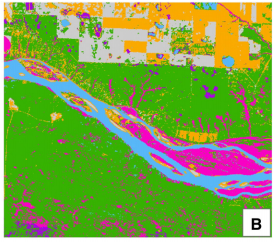
\includegraphics[width=\textwidth]{\dir/figs/pixel.png}
\caption{Pixel-wise decision tree}
\label{fig.pixel-based}
\end{subfigure}%
\qquad
\begin{subfigure}{0.35\textwidth}
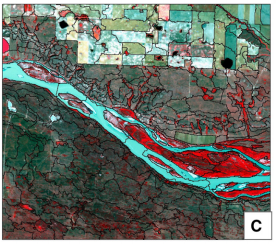
\includegraphics[width=\textwidth]{\dir/figs/mrs15_object.png}
\caption{Object-based using multi-resolution segmentation}
\label{fig.object-based}
\end{subfigure}
\caption{Comparison of image classification techniques, adapted from \cite{duro12}.}
\label{fig.pix_vs_obj}
\end{figure}
In object-based methods the pixels are grouped according to similar spectra and textural characteristics and then segmented (Figure \ref{fig.object-based}) (\cite{martha11}). The accuracy of this method is dependent on the thresholds that are manually adjusted for different cases, leading to uncertainties. In pixel-based classification (Figure \ref{fig.pixel-based}), the class is mapped pixel by pixel reducing the segmentation and need for manually defined thresholds (\cite{hussain13}). Some of these classification techniques look at the spectral characteristics of each pixel and assign it to a class. More advanced techniques combine information from neighbouring pixels in order to enhance the classifiers performance. These two pixel-based techniques are not viable on a large scale because they rely on the separability of different classes based on the spectrum of a single pixel or neighbouring pixels. In large scale satellite imagery, high spectral resolution is not always available so it becomes difficult to identify pixels based on their spectrum. Additionally, due to the large scale variability over entire datasets with high spatial extent, there are issues due to increased inter class variability (\cite{maggiori17b}).
\par
Due to the recent explosion in very high resolution imagery (VHR) there is now a need for an automatic classification method in order to reduce the processing time that is required for the current models. There are only a few semi-automated systems and no fully automated systems in existence (\cite{baltsavias04,mayer08,mnih13}). Deep learning therefore, is gaining traction as a method for pixel-based classification as it exploits feature representations based exclusively from data rather than handcrafted features that are designed based on domain-specific knowledge (\cite{xiao17,maggiori17a}). Convolutional Neural Networks (CNNs) are a deep learning technique that works to automatically discover relevant contextual features in image classification problems.
\par
\begin{figure}[b]
    \centering
    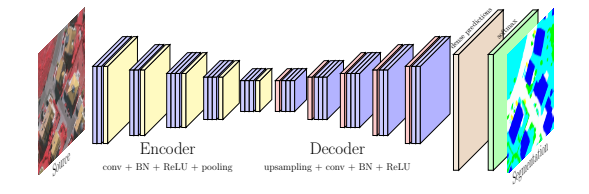
\includegraphics[width=0.9\textwidth]{\dir/figs/segnet.png}
    \caption{SegNet architecture for semantic labelling, taken from \cite{audebert18}}
    \label{fig.segnet}
\end{figure}
Convolutional Neural Networks (CNNs) have been inspired by the biological process as the network patterns resemble that of the animal visual cortex. They require relatively little pre-processing when compared to other classification algorithms, the network learns how to classify the image where in other classification algorithms the classifier needs to train the algorithm manually. Compared to other neural networks, CNNs have less connections and parameters and so are easier to train with their theoretical best performance only being slightly less (\cite{krizhevsky17}). The paper by \cite{long15} outlines how a fully convolutional neural network (FCN), that has been trained end-to-end, pixels-to-pixels, can exceed existing procedures (\cite{shelhamer17}). Figure \ref{fig.segnet} shows an example of the SegNet architecture to classify a scene using encoder-decoder to produce an output with the same resolution as the original scene (\cite{audebert18}). CNNs were designed for image classification tasks, i.e. assigning a single class label to an entire image (\cite{volpi17}). The first example of a successful CNN for image classification was a result of the ILSVRC challenge in 2012, where CNNs outperformed start-of-the-art classification systems (\cite{marmanis16,volpi17,krizhevsky17}).
